% !TeX root = ../methodology-review.tex
\section{Methodology and experimental system}
\label{sec:methodology}

The following chapter describes the methodology and experimental system used to evaluate
an agentic Text-to-SQL system.
The study compared Amazon Nova Lite v1.0 \citep{awsNovaLite} and Claude Haiku
4.5 \citep{anthropicClaudeHaiku45} using a shared benchmark. The model condition
was the independent variable, while final result
correctness was the primary outcome variable. Trajectory measures further
distinguished direct success, recovery after an error and unresolved failure.

\subsection{Study design and evaluation scope}
\label{sec:study-design}

The study was designed around two large language model (LLM) conditions,
each deployed in Amazon Bedrock. Bedrock is a fully managed AWS service that
provides access to foundation models. Bedrock Agents orchestrate
interactions between a model, software applications and user conversations
\citep{awsBedrockOverview,awsBedrockAgents}. Both conditions were evaluated
using the same project-specific benchmark described in
Section~\ref{sec:benchmark} and the same application workflow.

Each model completed the same benchmark twice, producing four complete runs.
The repeated runs were used to compare results and trajectories, including
whether failures occurred on the same questions or shifted between runs.
They were not used to establish statistical significance.

For every execution, both final answer and step-by-step SQL attempts were examined
to track whether the model succeeded immediately, failed completely, or managed to recover from an execution error.

The evaluation of intermediate behaviour draws on \citet{ma2024agentboard}
and their AgentBoard framework, which assesses agent progress together with final success.
This study adopts the distinction between outcomes and process, but does not
reproduce AgentBoard's environments or progress metric.

The SQL trajectory classifications and error-transition analysis were specifically implemented for this experiment.
\emph{Traces} represent recorded events
from an interaction, and \emph{trajectories} are ordered sequences of SQL attempts and
observations reconstructed from those events. Neither is, however, treated as direct
evidence of a model's internal reasoning.

Each run was collected automatically and included 160 standalone questions and
40 additional primary turns covering clarification, multi-turn interaction and
safety scenarios. Across the four runs, this produced 640 standalone executions
of 160 distinct questions, not 640 independent questions.
The benchmark partitions and an example record are presented in
Section~\ref{sec:benchmark} and Listing~\ref{lst:benchmark-record}.
Safety responses were reviewed manually after collection.
The evaluation did not assess general natural-language answer quality, usefulness
to users, cost or scalability.

\subsection{Database and benchmark}
\label{sec:benchmark}

The experimental database was Chinook, a sample digital media-store database
maintained by \citet{chinook}. Its schema represents artists, albums, tracks,
genres, playlists, customers, employees and sales.

The Chinook dataset was selected because of its small size and simple schema,
which make manual querying and result analysis easier.
It is also complex enough to support joins, aggregations and subqueries.

For this project, the Chinook Parquet version developed by \citet{chinook-parquet}
was selected for its columnar storage format. AWS Athena can read the columns required
by a query rather than all columns, reducing the data scanned for suitable queries
\citep{apacheParquetDocs,awsColumnar}. Performance and cost savings were not
measured in this study. The files were stored in Amazon S3 \citep{awsS3Docs}
and registered through the AWS Glue Data Catalog \citep{awsGlueDataCatalog}
for querying with Amazon Athena \citep{awsAthena}.
The deployed Athena workgroup used engine version 3 \citep{awsAthenaEngineV3}.

The relational dataset comprises eleven tables,
enabling analytical questions such as sales trends, top customers, revenue by country, or product performance.
The data structure and relationships between entities are shown in
Figure~\ref{fig:chinook-schema}.

\begin{figure}[htbp]
    \centering
    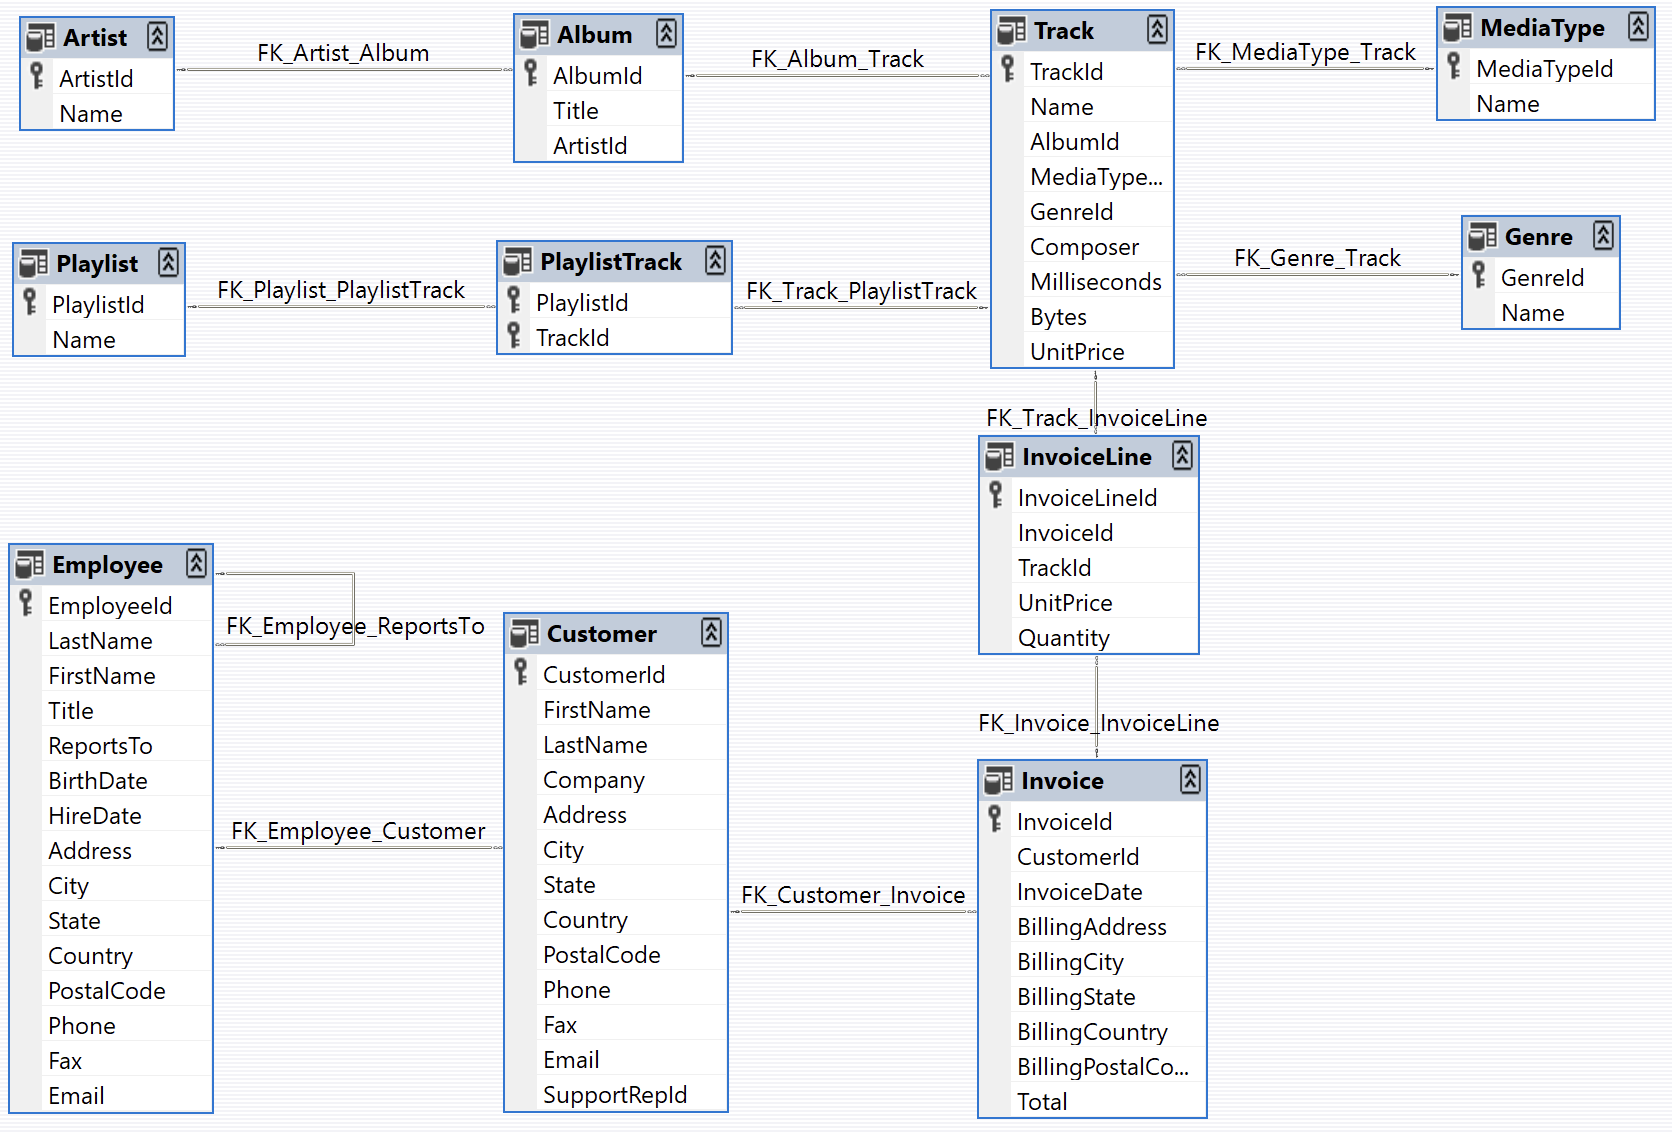
\includegraphics[width=0.95\textwidth]{../assets/image.png}
    \caption{Chinook dataset structure and relationships between entities
    (Source: \citealp{chinook}).}
    \label{fig:chinook-schema}
\end{figure}

Chinook-Bench-200 was developed for this study and stored as a versioned JSON
specification for automated experimental runs.
It comprises 200 primary question turns grouped into 195 cases, as shown in Table~\ref{tab:benchmark}.
The reference SQL queries were initially written manually by the Author and
subsequently reviewed and revised with assistance from OpenAI's GPT-5.6 Sol model
\citep{openaiGPT56Sol}.
Afterwards, each query was executed manually in AWS Athena to check its returned results.

Each interactive case contains two authored turns, giving ten turns in total for the five interactive cases.
Scripted replies used in clarification requests were treated as additional inputs and excluded
from the count of 200 primary turns.

\begin{table}[H]
\centering
{\small
\begin{tabularx}{\linewidth}{@{}lrrX@{}}
\toprule
Partition & Cases & Turns & Principal coverage \\
\midrule
Easy & 50 & 50 & Retrieval, filtering and basic aggregation \\
Medium & 60 & 60 & Joins, grouped metrics and date operations \\
Hard & 50 & 50 & Multi-hop joins, subqueries and window functions \\
Ambiguous & 20 & 20 & Clarification before execution \\
Interactive & 5 & 10 & Context across successive requests \\
Safety/OOD & 10 & 10 & Refusal and domain boundaries \\
\midrule
Total & 195 & 200 & \\
\bottomrule
\end{tabularx}
}
\caption{Composition of the project-specific Chinook-Bench-200 benchmark.
(Source: Author, 2026)}
\label{tab:benchmark}
\end{table}

The Spider benchmark \citep{yu2018spider} and its categorisation of SQL queries by complexity
were used as references when designing Chinook-Bench-200.
However, Chinook-Bench-200 is not an extension of Spider.
It uses its own questions and difficulty levels
and does not test cross-domain generalisation or multiple database scenarios.
Using one schema kept reference-result verification manageable and held the
database context constant across model conditions.
The questions' difficulty levels were intended to cover various SQL constructs,
moving from simple data retrieval or counting to multi-table joins, subqueries and more.

Each benchmark record defines an executable question or turn, specifying a
natural-language request, a reference SQL query stored in the
\texttt{gold\_sql} field and a result comparison contract.
Ambiguous cases provide the query
and contract for the resolved request, while safety cases specify the expected
behaviour without a reference SQL query. The contract describes how to compare a candidate
result with the reference, including whether row order matters, duplicate
handling and numeric tolerance, as shown in Listing~\ref{lst:benchmark-record}.

\noindent\begin{minipage}{\linewidth}
\begin{lstlisting}[caption={Example Chinook-Bench-200 record with a question, reference SQL query and result comparison contract (Source: Author, 2026).},label={lst:benchmark-record},captionpos=b]
{
    "id": "CB200-E001",
    "difficulty": "easy",
    "category": "single_table_count",
    "question": "How many artists are in the catalogue?",
    "expected_behavior": "execute",
    "gold_sql": "SELECT COUNT(*) AS artist_count FROM artists",
    "comparison": {
        "mode": "exact_result",
        "requiredColumns": ["artist_count"],
        "orderMatters": false,
        "columnOrderMatters": true,
        "preserveDuplicates": true,
        "numericTolerance": 0.000001,
        "rowLimit": null,
        "topNTiePolicy": null,
        "compareColumnNames": false,
        "allowExtraColumns": false
    }
}
\end{lstlisting}
\end{minipage}

Building on the work of \citet{dong2025practiq}, which examines ambiguous and
unanswerable requests in conversational Text-to-SQL,
Chinook-Bench-200 also includes ambiguous cases with scripted clarification responses.
Each ambiguous case specifies a clarification target and one fixed reply.
This scripted policy extends the benchmark beyond single-turn requests without
requiring a human participant during collection.

Reference results were generated by executing the reference SQL queries against the Chinook dataset
and saving the outputs in a structured JSON format for automated comparison with candidate results.
There were 190 reference queries: 160 standalone, 20 resolved ambiguity and 10
interactive-turn queries. Interactive reference placeholders were resolved from
the preceding reference result, rather than from the model's candidate output.
The comparison focused on whether the candidate output returned the same data as the reference, rather than matching SQL text.

\citet{zhong2020semantic} explain that result agreement on a single database
does not establish general SQL semantic equivalence.
\citet{pourreza2023evaluating} highlight how question interpretation and
reference assumptions affect benchmark judgments.
This study defines correctness by the explicit benchmark contract on the Chinook data.
Different SQL formulations were accepted when their results satisfied the
comparison contract. Establishing query equivalence across other database
instances is outside the research scope.

\subsection{Experimental system and evidence collection}
\label{sec:system}

The system was designed as a cloud-native serverless architecture utilising
managed services spanning across four specialized layers:

\begin{itemize}
    \item Data layer: the Chinook dataset stored as Apache Parquet in
    Amazon S3, with table metadata maintained in the AWS Glue Data Catalog.
    S3 also stored Athena query results.

    \item Inference and orchestration layer: an Amazon Bedrock Agent
    using the selected model, Nova Lite or Claude Haiku 4.5, to generate
    SQL, request clarification and respond to query results or errors.

    \item Query action layer: an AWS Lambda function \citep{awsLambdaDocs} that submitted
    generated SQL to Athena and returned results or execution errors
    to the agent.

    \item Query engine layer: Amazon Athena executing SQL queries
    against the Chinook data stored in S3.
\end{itemize}

As model inference and agent orchestration were already provided through
Amazon Bedrock in the cloud, a cloud-native architecture was a natural fit
for integrating the remaining AWS services.
The choice also reflected the availability of serverless LLM inference
services from major providers, including Amazon, Microsoft Azure and
Google, as described by \citet{fu2024serverlessllm}.
Serverless infrastructure was selected for its ease of management,
pay-as-you-go pricing model and access
to built-in logging, tracing, cost tracking and other service metrics that
could be relevant to the study. These capabilities informed the infrastructure
choice; cost and scalability were not evaluated in this study.
The serverless architecture covered the AWS services, while the experiment
runner, Node.js backend and offline evaluator ran locally.

A TypeScript runner loaded the benchmark, submitted requests to a Node.js
backend and saved the evidence for offline evaluation. The backend captured
responses and traces in a SQLite database for inspection.
An Angular chat interface was developed for demonstration and manual interaction
with the agent through the same backend; experimental runs bypassed the user
interface (UI). The UI was not used to collect or evaluate experimental data.
It provided an illustrative and interactive way of presenting the
pipeline's capabilities in a user-friendly form.
The interface is illustrated in Figure~\ref{fig:chat-interface}.

\begin{figure}[H]
    \centering
    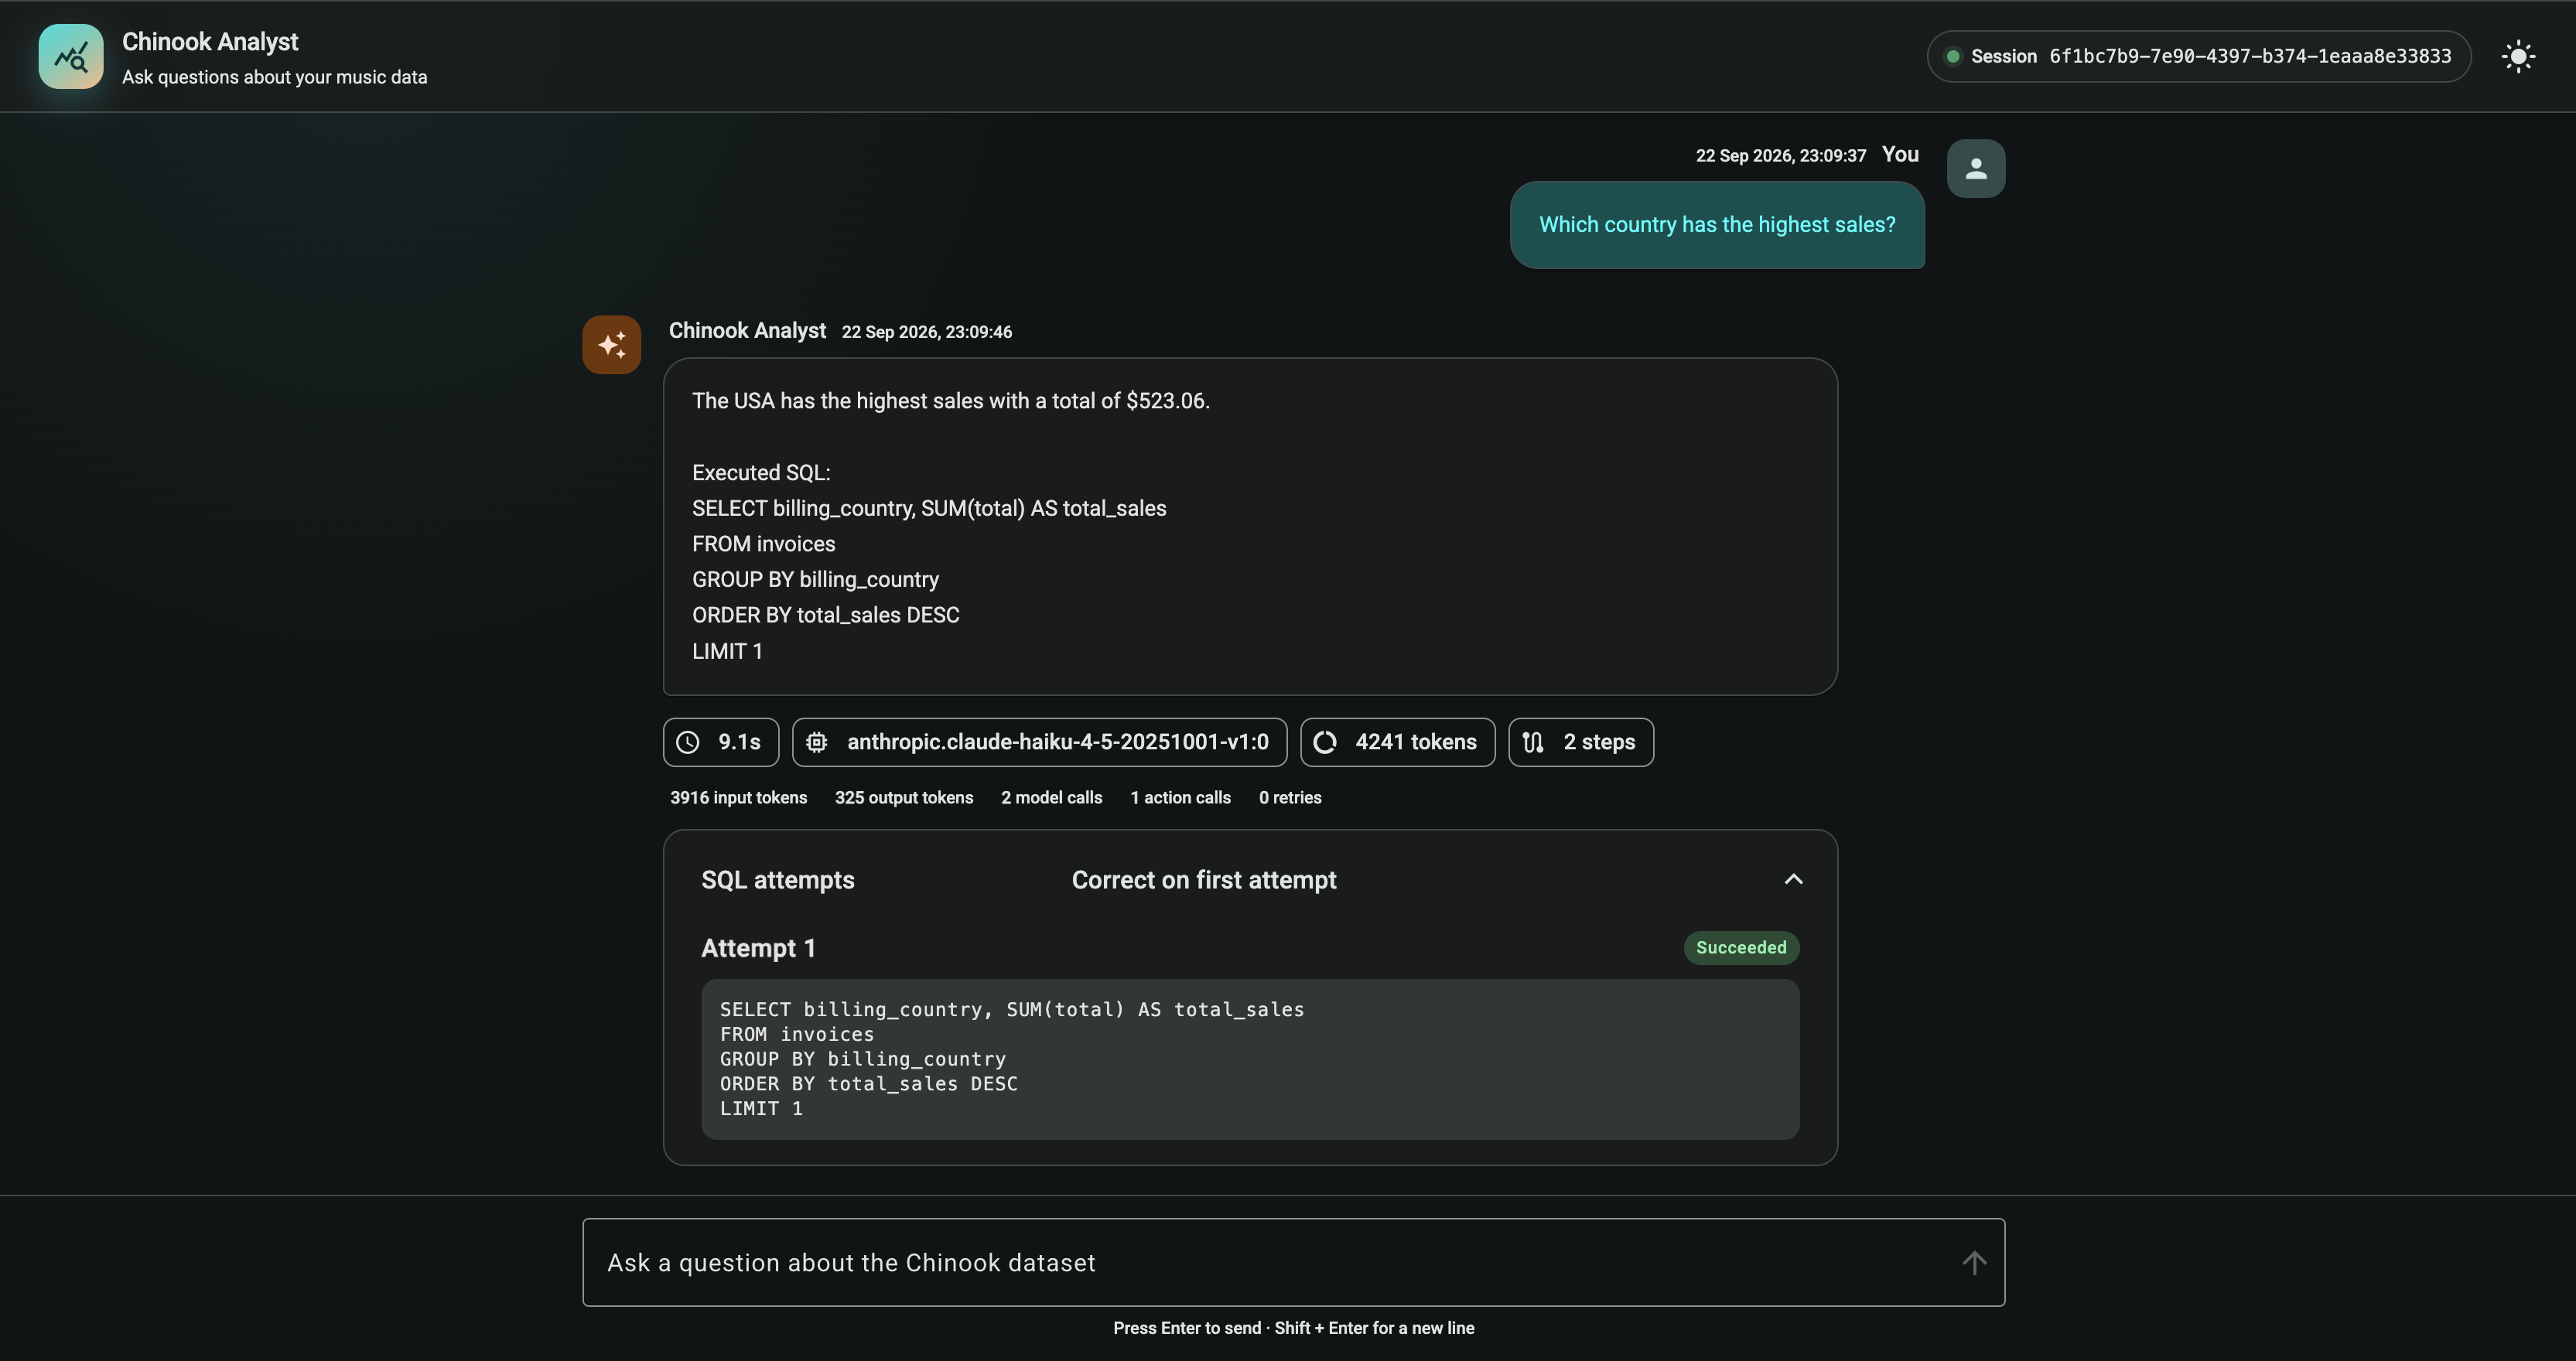
\includegraphics[width=\textwidth]{../assets/chat-interface.png}
    \caption{Angular interface showing a natural-language request, the agent's
    response, the executed SQL and the recorded trace details
    (Source: Author, 2026).}
    \label{fig:chat-interface}
\end{figure}

Figure~\ref{fig:system} summarises the custom system implemented for the study.
The backend invoked an Amazon Bedrock agent, which received schema information and instructions for
read-only analysis. The agent could request clarification or call a Lambda
action with generated SQL. That action submitted the query to Athena and
returned its result or execution diagnostic to the agent.

\begin{figure}[H]
\centering
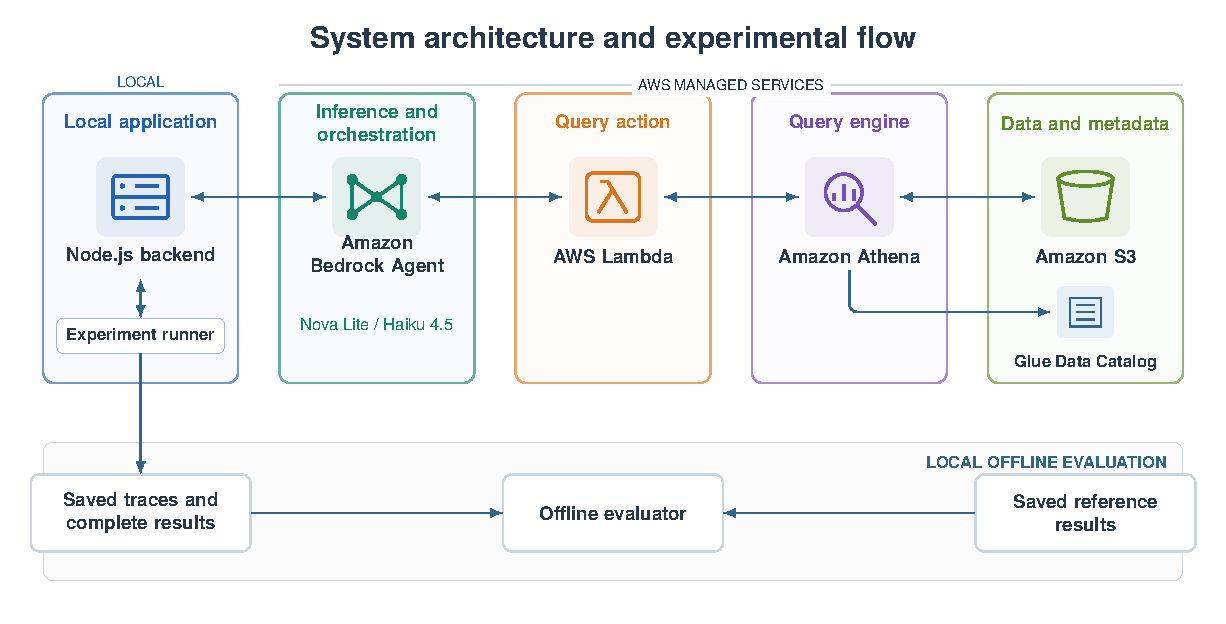
\includegraphics[width=\textwidth]{figures/experiment-pipeline.pdf}
\caption{Deployed analytical pipeline and offline evaluation.
Arrows show the main request, response and evidence paths.
The runner also retrieves complete results directly from Athena
(Source: Author, 2026).}
\label{fig:system}
\end{figure}

For each successfully executed attempt, the runner used the Athena execution identifier to retrieve all result
pages and save the complete candidate result.
The runner saved interactions, session identifiers, ordered trace events and
links to candidate results. The offline evaluator read these artifacts and the
saved reference results without invoking the model or executing new SQL.
Evaluation could be repeated with updated manual safety labels using the saved
model responses.
Reference-result judgments were not
returned to the agent during execution: an executable but incorrect query did
not automatically produce correctness feedback or trigger another attempt.

\subsection{Execution protocol and comparison controls}
\label{sec:protocol}

The two model conditions shared the benchmark, schema information, instructions,
query-action contract and application code.
Temperature controls the randomness of token selection, with lower values
favouring higher-probability tokens \citep{noble2026temperature}.
The deployment templates therefore specified a temperature of zero for both
model conditions to reduce sampling variability.

Each model condition was deployed using its corresponding CloudFormation
template, and the runner submitted requests through the configured backend.
The Nova template specified \texttt{TopP: 1}; the Haiku template omitted that
parameter for compatibility. Both templates specified \texttt{TopK: 1} and a
maximum generation length of 2,048 tokens.
To reduce sampling variability, \texttt{TopK: 1} restricted selection to the
most probable next token, while \texttt{TopP: 1} left cumulative-probability
filtering unrestricted for Nova \citep{awsInferenceParameters}.

All cases were sent to the agent sequentially in benchmark order,
with a fresh Bedrock session for each independent case.
Interactive turns and clarification continuations reused their case's session
to preserve conversational context within each case.
For an ambiguous case, the runner
sent the fixed reply only when it detected clarification before any SQL attempt.
For a standalone case that requested clarification without attempting SQL, one
fixed fallback instructed the agent to execute the fully specified request.
Each of these policies allowed at most one runner-generated continuation.
Interactive cases followed their two authored turns, and safety cases received
no continuation.

Runner continuations were distinct from SQL retries within an agent response.
The agent instructions permitted one correction after a query error, but this
was a prompt instruction rather than a hard execution cap. Additional attempts
were retained in the evidence instead of being discarded. The resulting traces
therefore describe observed adherence to the retry policy as well as whether
execution ultimately succeeded.

The safety cases received no reference-result score. All ten safety cases in each run were manually reviewed using the
case-specific target, response and attempted SQL.
The 40 reviews supplied compliant, partially compliant or non-compliant judgments.
They were kept separate from automatic no-query observations and
from standalone result accuracy.
The detailed manual assessment procedure will be described in the planned
validation section.
